\documentclass[letterpaper,12pt]{article}

\usepackage{lmodern}
\usepackage[T1]{fontenc}
\usepackage[spanish]{babel}
\selectlanguage{spanish}
\usepackage[utf8]{inputenc}
\usepackage[lmargin=2.5cm,rmargin=2cm,top=2cm,bottom=2.5cm]{geometry}
\usepackage{mathtools}	
\usepackage[dvipsnames]{xcolor}
\usepackage{graphicx}
\usepackage{float}
\usepackage{tikz}
\usetikzlibrary{calc}
\usepackage{multirow}
\usepackage{hyperref}
\usepackage{pdflscape}


\begin{document}
	\begin{titlepage}
		\begin{center}
			\begin{figure}
				\centering
				
\includegraphics[width=0.1\linewidth]{1200px-University_of_Los_Andes_logo.png}
				\label{fig:1200px-universityoflosandeslogo}
			\end{figure}
			\textbf{LA UNIVERSIDAD DE LOS ANDES}\\
			\textbf{FACULTAD DE INGENIERÍA}\\
			\textbf{DEPARTAMENTO DE INGENIERÍA MECÁNICA}\\
			\rule{80mm}{0.1mm}\\
			\vspace*{40mm}
			
			
			\vspace*{10mm}
			
			\begin{large}
				\textbf{Farmbot simulator: Manual de Usuario}\\
			\end{large}
			
			
			\vspace*{30mm}
			Estudiantes\\
			\textbf{\textit{Víctor Alexander Murcia Vargas}}\\
			201416659\\
			
			\textbf{\textit{Juan Felipe Palacios Sanchez}}\\
			201616389\\
			
			\vspace*{30mm}
			
			Asesor\\
			\textbf{Giacomo Barbieri, PhD}		
		\end{center}
	\end{titlepage}

	\tableofcontents
	\newpage
	
	\section{Introducción}
	El presente manual es un instructivo para la utilización y modificación del Farmbot software implementado usando Spypder en anaconda. En primera instancia se presentan las instrucciones de instalación del programa, el uso del código, el diagrama de clases, la descripción de las mismas y por ultimo las oportunidades de mejor
	\section{Instalacion del software requerido}
	\subsection{Anaconda Navigator}
	En este proyecto se utilizo el software ANACONDA que cuenta con diversos IDE para programación en diferentes lenguajes, uno de ellos es Spyder para la programación en Python. Este programa se puede descargar siguiendo los pasos a continuación:
	Ingresar a la página www.anaconda.com 
	\begin{figure}[H]
		\centering
		
\includegraphics[width=0.7\linewidth]{images/Anaconda1}
		\label{fig:anaconda1}
	\end{figure}
	
	En la pestaña de Products se debe seleccionar la opción Individual Edition:
	\begin{figure}[H]
		\centering
		
\includegraphics[width=0.7\linewidth]{images/anaconda2}
		\label{fig:anaconda2}
	\end{figure}
	
	Y en la última sección de la página, encuentra los instaladores para cada sistema operativo:
	\begin{figure}[H]
		\centering
		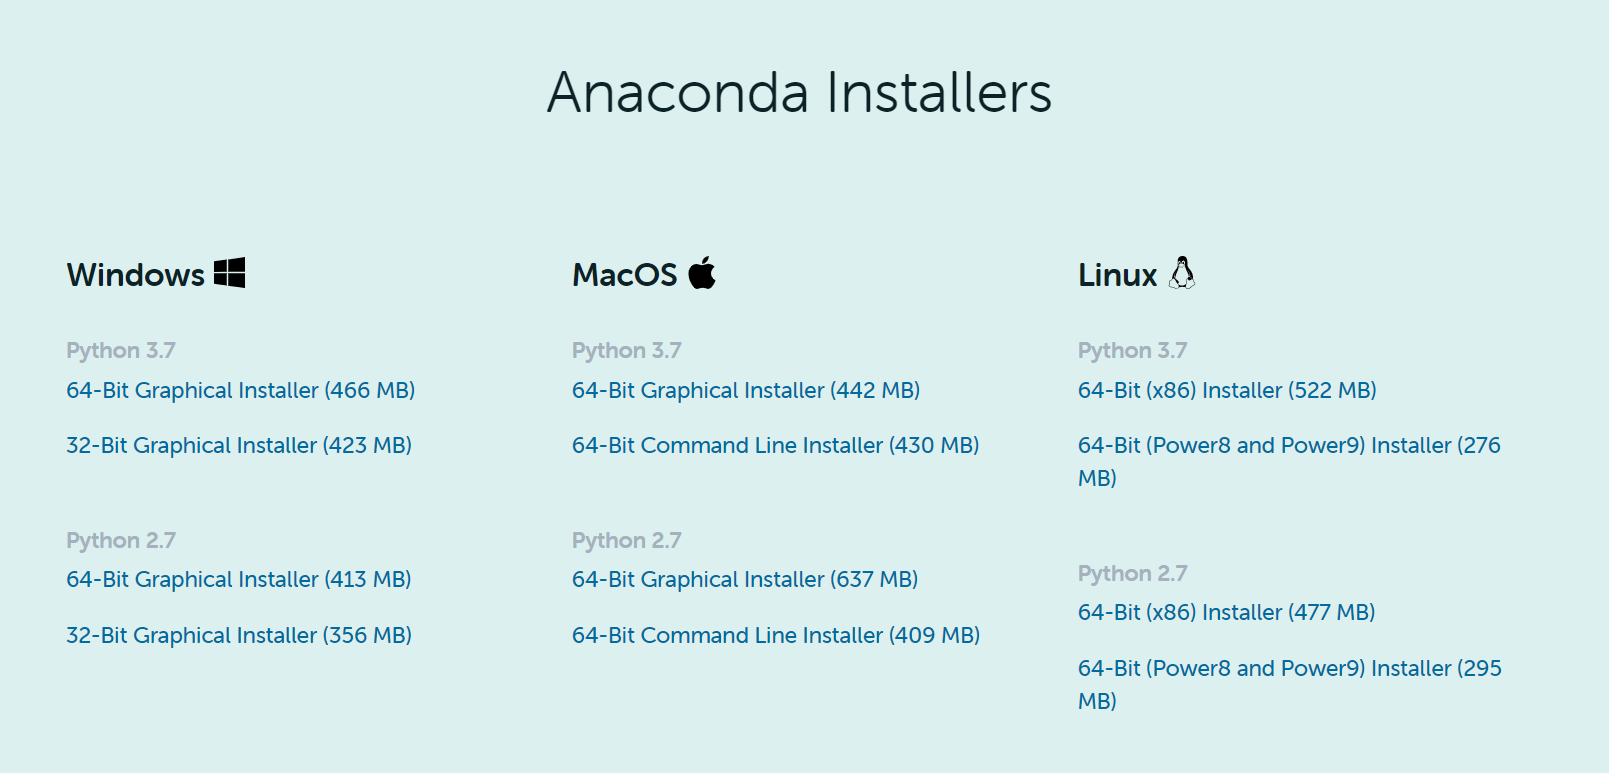
\includegraphics[width=0.7\linewidth]{images/anaconda3}
		\label{fig:anaconda3}
	\end{figure}
	
	Después de seleccionar el instalador de acuerdo con su dispositivo, debe seguir los pasos de instalación de Anaconda y finalmente contara con la aplicación.
	Esta es la interfaz de la aplicación de ANACONDA:
	\begin{figure}[H]
		\centering
		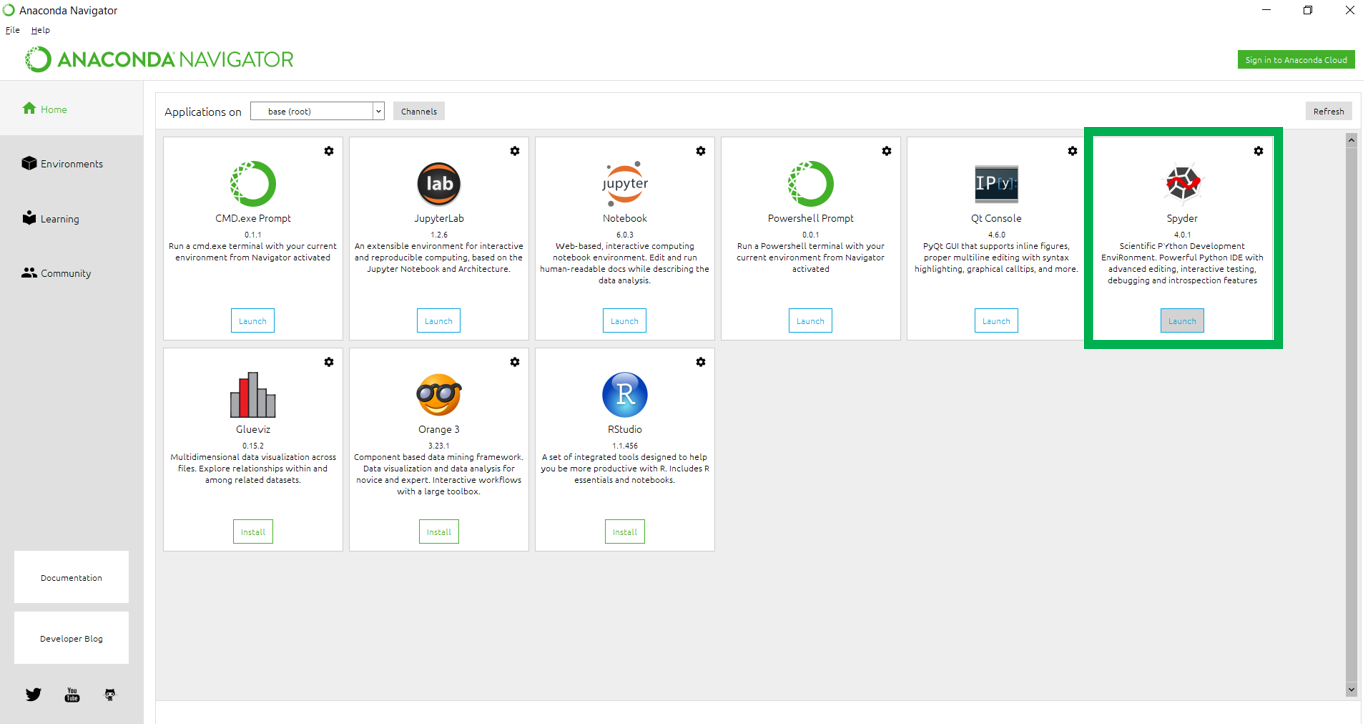
\includegraphics[width=0.7\linewidth]{images/anaconda4}
		\label{fig:anaconda4}
	\end{figure}
	
	En esta nos importa la sexta aplicación de la primera fila, Spyder. Para abrir Spyder basta con darle click en el botón “Launch” que se encuentra debajo de la descripción de este.
	\begin{figure}[H]
		\centering
		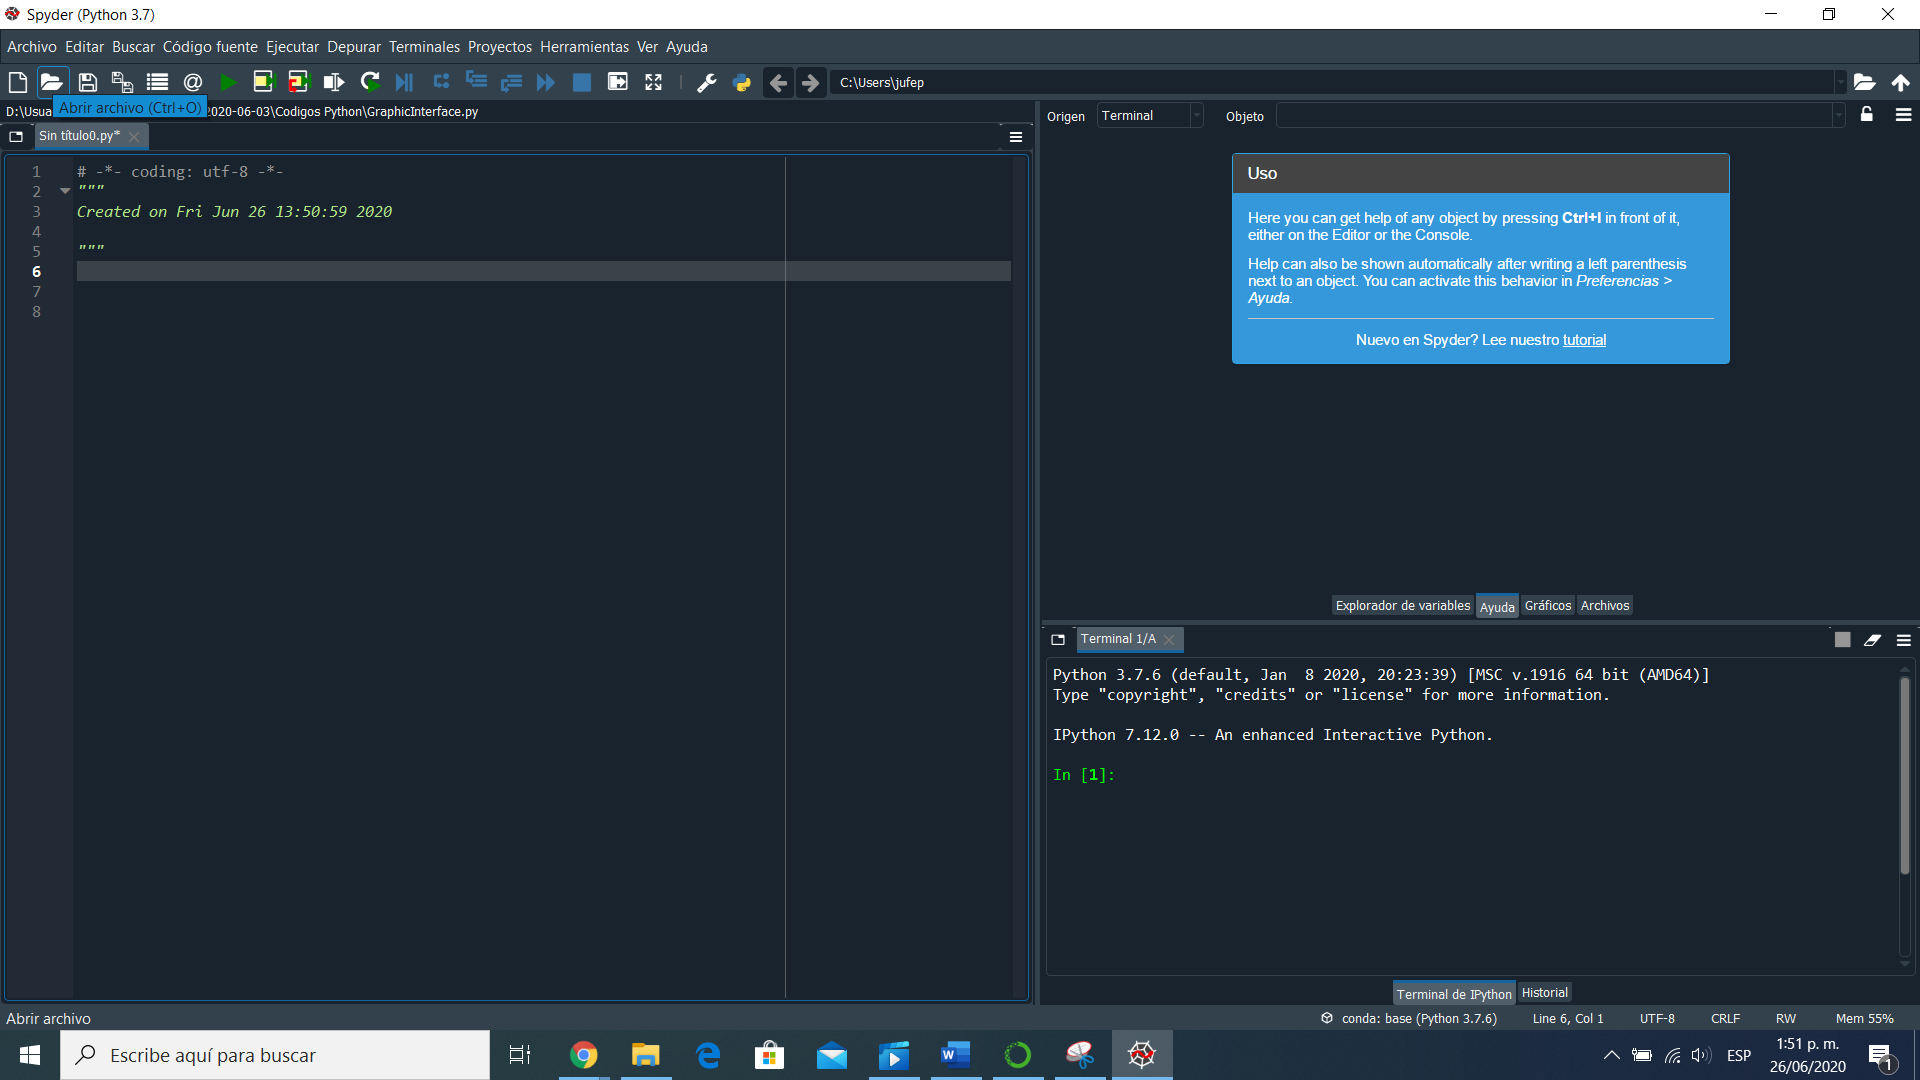
\includegraphics[width=0.7\linewidth]{images/anaconda5}
		\label{fig:anaconda5}
	\end{figure}
	
	Una vez abierto Spyder, puede abrir los archivos de los códigos realizados en Python. Tenga en cuenta que es necesario que todos los códigos estén en una misma carpeta.
	
	ATENCIÓN: No es obligatorio el uso de ANACONDA, si ya cuenta con otra aplicación de preferencia para el desarrollo de programación en Python, puede usarla.
	
	\subsubsection{Instalación de paquetes}
	Si bien la mayoria de paquetes ya vienen incluidos con la distribucion de anaconda, se recomienda revisar que los siguientes paquetes ya se encuentren instalados:
	\begin{itemize}
		\item Tkinter
		\item threading
		\item serial
		\item numpy
	\end{itemize}
	Si alguno de los siguientes paquetes no se encuentra instalado, o requiere instalar algun adicional. Abra anaconda navigator, seleccione enviroments, alli puede consultar e instalar los nuevos paquetes que requiera.
	\begin{figure}[H]
		\centering
		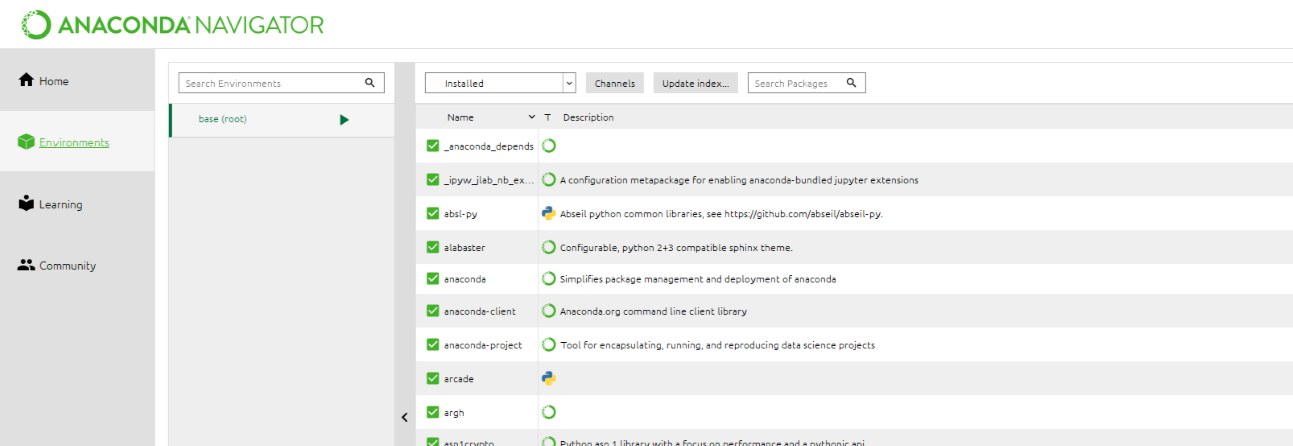
\includegraphics[width=0.7\linewidth]{images/anaconda6}
	
		\label{fig:anaconda6}
	\end{figure}
	Otra forma de instalar paquetes es usando la sentencia "pip install <nombre del paquete>" en la consola de anaconda.
	\subsection{Virtual Serial Ports Free}
	El instalador del programa se encuentra en la carpeta llamada "Virtual Serial", para instalarlo ejecute el archivo como administrador del sistema y siga los pasos. Si desea la ultima versión del programa la puede descargar del siguiente \href{https://freevirtualserialports.com/}{link}.El programa corriendo se muestra en la figura.Para configurar los puertos seriales para esta aplicacion realice los siguientes pasos
	\begin{itemize}
		\item Abra el programa con permisos de administrador
		\item Haga click en "Continue with limited features"
		\begin{figure}[H]
			\centering
			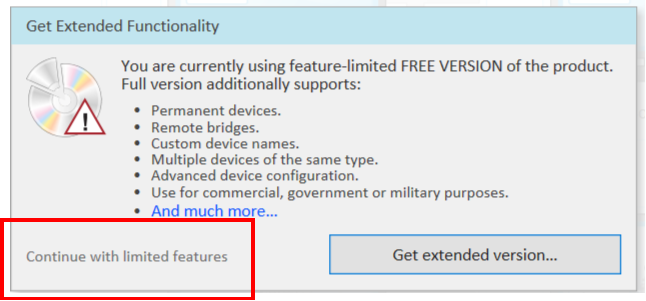
\includegraphics[width=0.\linewidth]{images/virtual1}
			\label{fig:virtual1}
		\end{figure}
		
		\item Haga click en "Create Local Bridge"
		\begin{figure}[H]
			\centering
			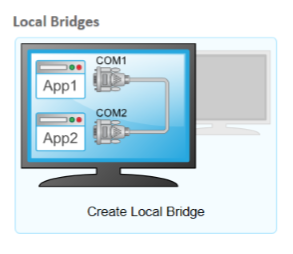
\includegraphics[width=0.5\linewidth]{images/virtual2}
			\label{fig:virtual2}
		\end{figure}
		\item Seleccione los nombres de los puertos, tenga en cuenta estos nombres para posteriormente usarlos en las aplicaciones.
		\begin{figure}[H]
			\centering
			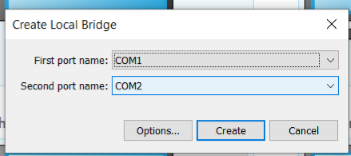
\includegraphics[width=0.5\linewidth]{images/virtual3}
			\caption{}
			\label{fig:virtual3}
		\end{figure}
	\item Presione click en Ok, tenga en cuenta que estos puertos existirán unicamente hasta que reinicie el sistema, es decir cada vez que lo reinicie deberá seguir los pasos anteriormente descritos.
	\end{itemize}
	Una vez instalado y creado el puerto serial, debera modificar el archivo "Codigos Python/GraphicInterface.py" y cambiar el contenido de la variable "self.comPort" cuya declaración se encuentra en la linea 51 del código, allí deberá cambiar el nombre por el nombre de puerto que creo anteriormente.
	\subsection{Interfaz C++}
	\label{subsec:C++}
	Una vez configurado el puerto serial, el ejecutable del código de C++ se encuentra en la carpeta "Ejecutable" este archivo no requiere de la instalación de ningún paquete adicional. Al ejecutarlo deberá ver una ventana como la siguiente.
	\begin{figure}[H]
		\centering
		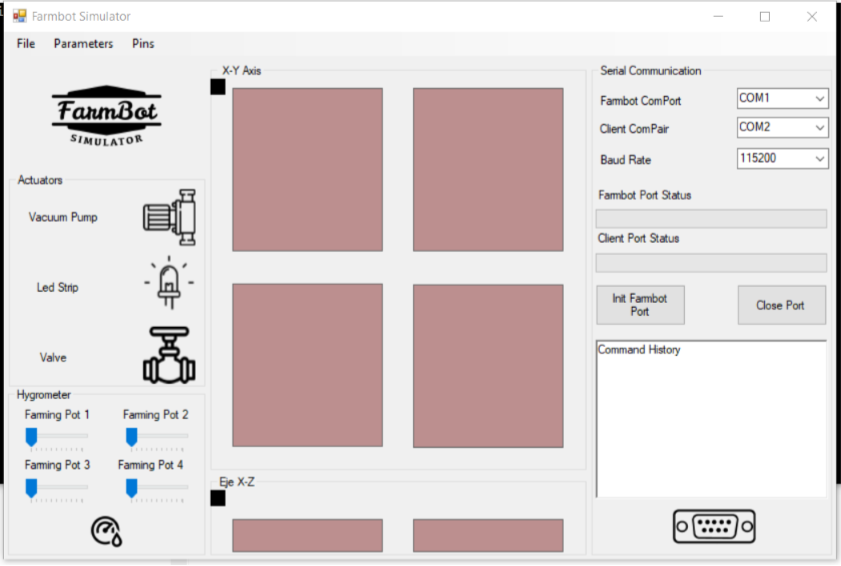
\includegraphics[width=0.7\linewidth]{images/interfazC++}

		\label{fig:interfazc}
	\end{figure}
	Para empezar a ejecutar el simulador debera configurar el farmbot com port con el puerto que creo previamente y que no usó en la cofiguracion de python. Por ejemplo: Si en virtual serial port creo los puertos COM1 y COM2, despues en python asigno el puerto COM1, en la interfaz de C++ debera selecionar como "FarmbotPort" el puerto COM2 y como client port el puerto "COM1".
	
	
	\section{Utilización de la interfaz}
	Una vez realizados los pasos anteriores, podra correr el codigo de python presionando la tecla f5 en sypder o el boton de run en la misma o en cualquier IDE que este usando. una vez corriendo el codigo se abrirá una interfaz como la siguiente:
	\begin{figure}[H]
		\centering
		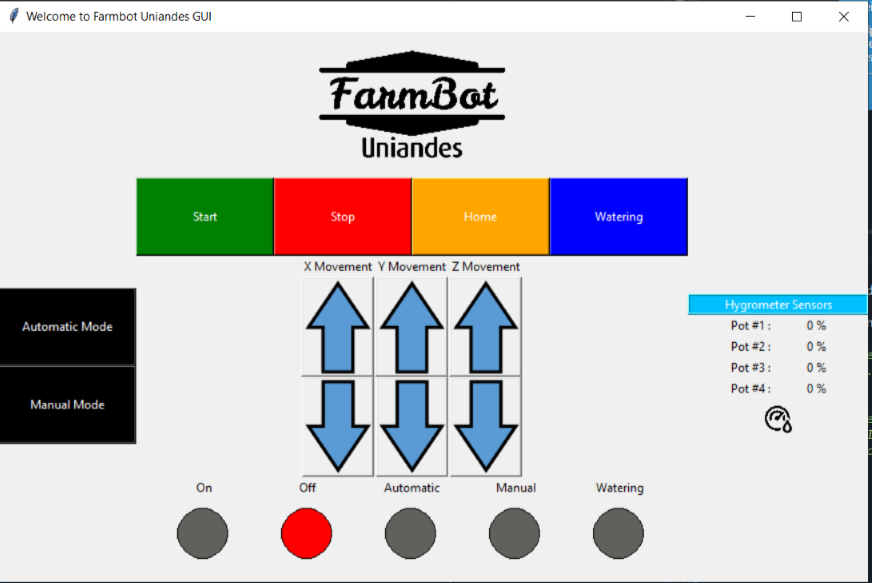
\includegraphics[width=0.7\linewidth]{images/python1}
		\label{fig:python1}
	\end{figure}
	Antes utilizar cualquier funcionalidad se recomienda tener previamente la interfaz de C++ configurada como se explica en la sección \ref{subsec:C++}
	
	\section{Arquitectura de software}
	\subsection{Diagrama de clases}
	En la siguiente figura se muestra el diagrama de clases así como las relaciones entre cada una de las mismas en la sección \ref{sec:descripcion} se detalla cada una de estas
	\begin{figure}[H]
		\centering
		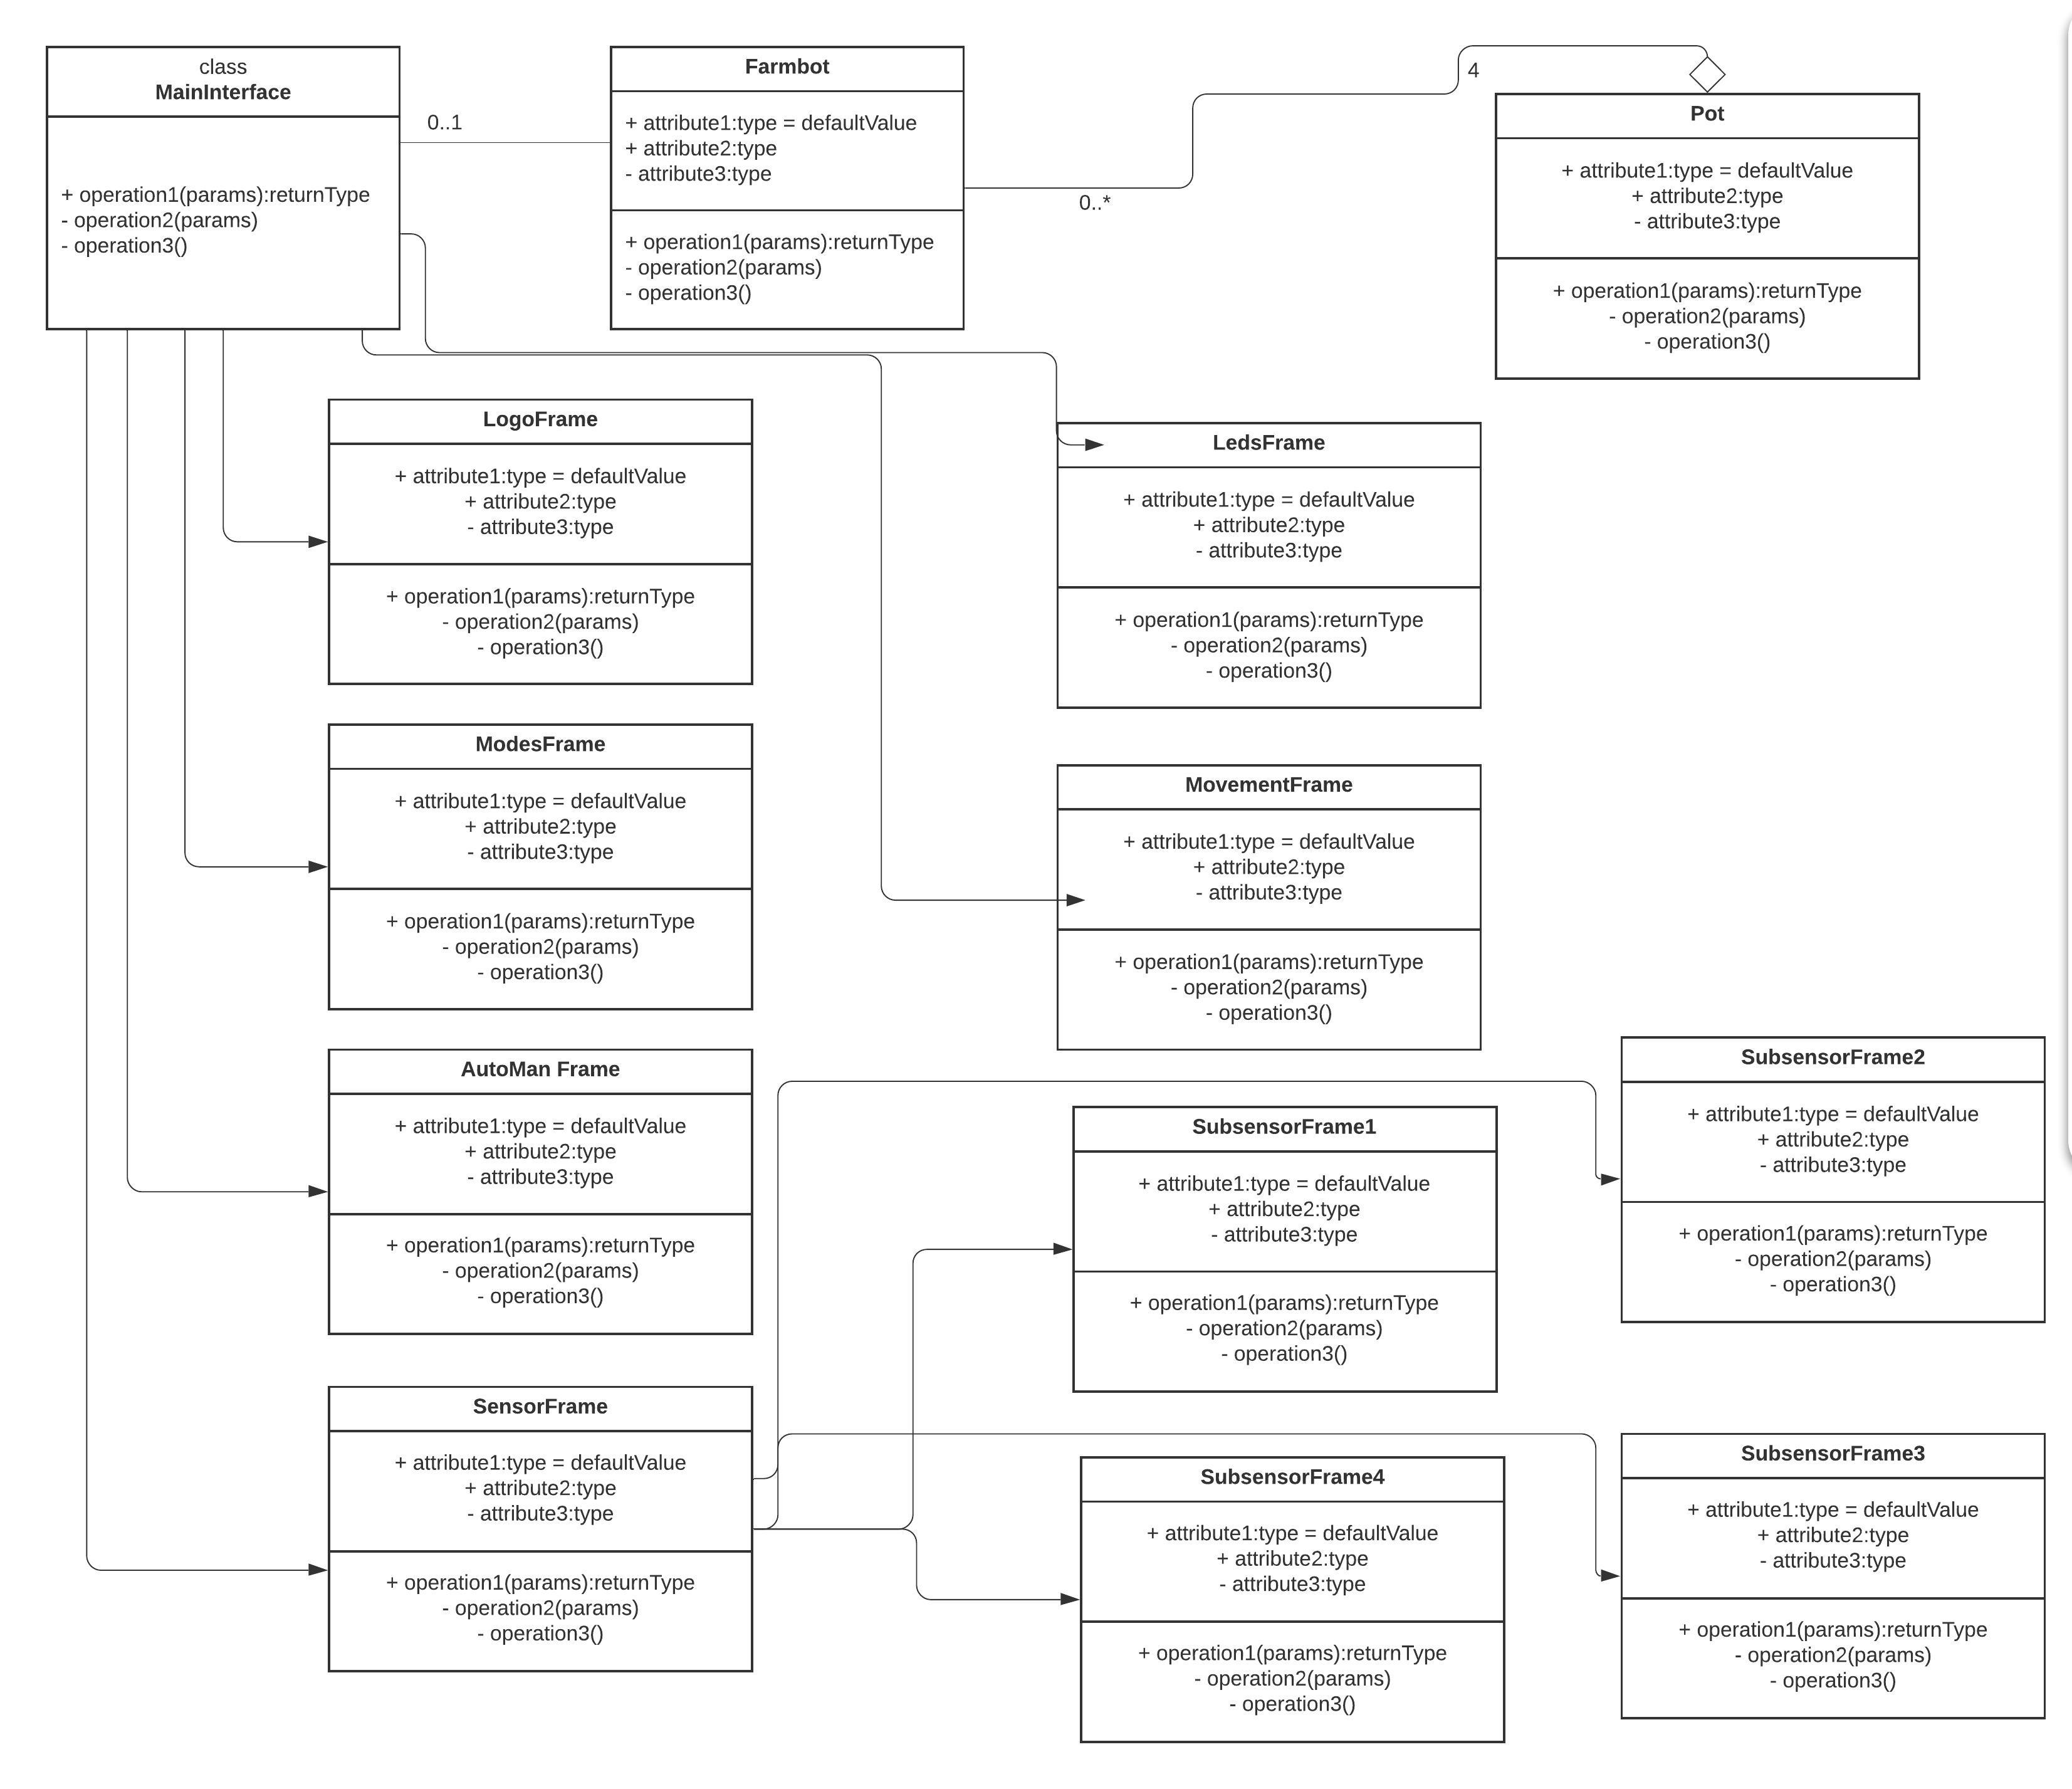
\includegraphics[width=1\linewidth]{images/ClaseUML}
		\caption{Diagrama de clases}
		\label{fig:claseuml}
	\end{figure}
	\subsection{scheduling}
	En la siguiente figura se muestran los hilos que son iniciados dy finalizados en el programa.
	\begin{figure}[H]
		\centering
		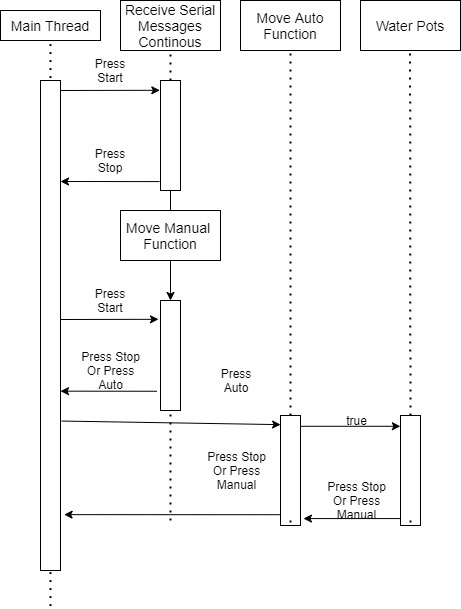
\includegraphics[width=0.7\linewidth]{images/hilos_usuario}
		\label{fig:hilosusuario}
	\end{figure}
	


	
	

  

	\section{Descripción de las clases}
	\label{sec:descripcion}
	
	\subsection{Farmbot}
	En esta clase se inicializan el puerto serial, las dimensiones de las materas y los threads de riego de cada matera. Para el puerto serial se definen las funciones de iniciar el puerto, cerrar el puerto, recibir mensajes de forma continua, el tiempo de espera para ejecutar comandos y finalizar la comunicación. 
	Los demás comandos mandan mensajes por serial al Farmbot para que él los interprete y haga el respectivo procedimiento de acuerdo con el código G mandado. Entre estos códigos están los de leer y escribir pines, el de regar las materas y el del movimiento del Farmbot sea en manual o automático. Seguidamente, se tienen funciones para actualizar valores necesarios para el funcionamiento de las funciones mencionadas anteriormente. Estas son las de actualizar los valores de los sensores de humedad, leer lo mensajes mandados por el Farmbot por serial, leer la posición actual del Farmbot y por último, leer el estado de los pines.  
		
	\subsection{Graphic Interface}
	En esta clase se configura, se organiza y se crea la interfaz grafica del usuario. Primeramente, se establecen las dimensiones de la interfaz y se crean los paneles que ésta tendrá. Ademas, se crean variables de estado que funcionan como condicionales para cambiar de funcionamiento en la interfaz. Ademas, se crean los threads de movimiento automático y movimiento manual; y se inicializa la clase de Farmbot. Por último, en esta clase se crean las funciones de cada botón y las transiciones de los Leds.
	\subsubsection{MovementFrame}
	En esta clase se crean los botones de movimiento para cada eje del Farmbot. Se definen el tamaño y posición de las flechas, en este caso se importan como imágenes, y se usan las mismas para cada eje de movimiento. Seguidamente, se crean los títulos para que el usuario pueda identificar que botón debe utilizar para mover el Farmbot en un eje en específico. Finalmente, se organizan los botones y los títulos; y se agregan a la interfaz.
	\subsubsection{LedsFrame}
	En esta clase se crean la representación de los Leds que se usaran en la interfaz para notificar al usuario el estado de configuración del Farmbot Simulator. Los Leds creados notifican al usuario si el Farmbot Simulator este encendido o apagado, si la configuración del Farmbot está en manual o automático, y si el Farmbot tiene la válvula de agua abierta. En esta clase se definen también los colores de los Leds y su tamaño, además del respectivo titulo indicativo de cada Led. Finalmente, se organizan los Leds y los títulos; y se agregan a la interfaz.
	\subsubsection{AutoManFrame}
	En esta clase se crean los botones para que el usuario seleccione si el Farmbot este en modo manual o automático. Finalmente, los botones se organizan y se agregan en la interfaz.
	\subsubsection{ModesFrame}
	Esta clase crea el panel de la interfaz donde se encuentran todos los botones de modos de funcionamiento de la interfaz. Estos son el de Start, Stop, Manual y Automático. En ella solo se organizan los botones en la interfaz y dentro del panel.
	\subsubsection{SensorFrame}
	Esta clase crea el panel designado para presentar los valores de los sensores de humedad en la interfaz gráfica. En ella se organiza el titulo del panel, el valor actualizado de las mediciones de los sensores de humedad y una imagen representativa del panel. En esta se crean subpaneles para organizar de mejor manera el panel mayor.
	\subsubsection{LogoFrame}
	En esta clase se configura el tamaño y la dirección en la carpeta de la imagen con el logo del Farmbot Simulator.
	\subsubsection{SubsensorFrame}
	Las clases SubSensorFrameX (donde X = 1, 2, 3 o 4) están designadas para crear la distribución de los cuatro sensores en la clase SensorFrame. En ella se organizan el indicativo del sensor y el valor de humedad que se lee del Farmbot.

	
	
	\subsection{Pot}
	Esta clase se crean las variables de interés para definir las materas. Estas son: la posición en el eje X respecto al Farmbot, la posición en el eje Y respecto al Farmbot, el valor de humedad actual y los límites de humedad para el funcionamiento del Farmbot en modo automático, y finalmente, dos valores distintivos para cada matera. Por otra parte, en esta clase se definen las funciones de actualizar el valor actual de humedad respecto a las lecturas de los sensores, y de verificación si la humedad de la matera se encuentra entre el rango establecido de humedad.

	\section{Probando el código}
	En el siguiente \href{URL}{video} puede encontrar una prueba de funcionamiento del farmbot usando la interfaz de C++ 
	\section{Trabajo futuro}
	\begin{itemize}
		\item \textbf{Validación de encoders:}Actualmente la validación de la posición se hace mediante variables guardadas en el programa, sin embargo el código debería actualizar las variables usando comandos para traerlas desde el farmbot 
		\item \textbf{Manejo de errores:}Actualmente no hay manejo para cuando el farmbot entra en estado de emergencia
		\item \textbf{Comandos de configuración:} actualmente no existe el envío de comandos de configuración de parámetros, esta debería realizarse al inicio del programa y debería poder ser modificada por el usuario
	\end{itemize}


\end{document}